\subsection{Model Organization}
The package diagram can be seen in figure \ref{fig:pkg}. Observing the Figure indicate that the top level is named PSOS (Particle Swarm Optimization System), note that the other packages connect to this namespace.\\

A brief description of the content:
\begin{itemize}
	\item \nameref{requirementspecification:operation} contains Use Cases and Requirements diagrams, see section \ref{requirementspecification:operation} \nameref{requirementspecification:operation}, page \pageref{requirementspecification:operation}.
	\item \nameref{requirementspecification:Structure} contains Block Definition and Internal Block diagrams, see section \ref{requirementspecification:Structure} \nameref{requirementspecification:Structure}, page \pageref{requirementspecification:Structure}.
	\item \nameref{requirementspecification:Behavior} contains Activity, Sequence and State Machine diagrams, see section \ref{requirementspecification:Behavior} \nameref{requirementspecification:Behavior}, page \pageref{requirementspecification:Behavior}.

\end{itemize}

\begin{figure}[H]
	\centering
	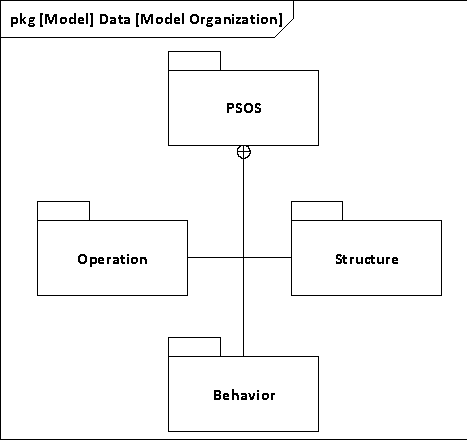
\includegraphics[width=0.5\linewidth]{diagram/pkg_data_model_organization.pdf}
	\caption{Package Diagram with the namespace PSOS}
	\label{fig:pkg}
\end{figure}